
%(BEGIN_QUESTION)
% Copyright 2006, Tony R. Kuphaldt, released under the Creative Commons Attribution License (v 1.0)
% This means you may do almost anything with this work of mine, so long as you give me proper credit

The relationship between the amount of voltage produced by a thermocouple's measurement junction ($E_{meas}$), the voltage produced by the reference junction ($E_{ref}$), and the voltage received by the measuring instrument ($E_{meter}$) is stated by the following equation:

$$\includegraphics[width=15.5cm]{i00385x01.eps}$$

$$E_{meter} = E_{meas} - E_{ref}$$

In a {\it hardware-compensated} thermocouple measuring instrument, the reference junction's voltage is canceled by the addition of a variable voltage source inside the instrument which we will designate as $E_{comp}$.  An alternative approach is to connect an external device called an {\it electronic ice-point} between the voltage-measuring instrument and the thermocouple, such that the ``ice point'' device adds the necessary voltage to compensate for the reference junction:

$$\includegraphics[width=15.5cm]{i00385x03.eps}$$

Re-write the thermocouple circuit equation to include this ``compensating'' voltage, and identify both the magnitude and the polarity this voltage must have in order to successfully cancel $E_{ref}$.

\vskip 20pt \vbox{\hrule \hbox{\strut \vrule{} {\bf Suggestions for Socratic discussion} \vrule} \hrule}

\begin{itemize}
\item{} Why can't we just somehow build the thermocouple circuit so it doesn't have a reference junction at all?  That way we wouldn't have to concern ourselves with compensation for this junction!
\item{} Should we use thermocouple extension wire to connect the voltmeter to the ice-point circuit, or is copper wire sufficient?
\item{} Can we get away with using copper extension wire all the way to the thermocouple so long as we're using an ice-point circuit?  Why or why not?
\end{itemize}

\underbar{file i00385}
%(END_QUESTION)





%(BEGIN_ANSWER)

\noindent
{\bf Partial answer:}

$$E_{meter} = E_{meas} - E_{ref} + E_{comp}$$

%(END_ANSWER)





%(BEGIN_NOTES)

Compensating voltage magnitude:

$$E_{comp} = E_{ref}$$

\vskip 10pt

Compensating voltage polarity:

$$\hbox{\it Opposite that of }E_{ref}$$

\vskip 10pt

Effect of compensating voltage addition:

$$E_{meter} = E_{meas} - E_{ref} + E_{comp}$$

$$E_{meter} = E_{meas} + 0$$

$$E_{meter} = E_{meas}$$


$$\includegraphics[width=15.5cm]{i00385x02.eps}$$

$$\includegraphics[width=15.5cm]{i00385x04.eps}$$

%INDEX% Measurement, temperature: thermocouple

%(END_NOTES)


